\begin{frame}{Overview} 

    This work is inspired by by the planar zero-sum pursuit-evasion game between 2 agents [1].  
    % 
    \begin{figure}
        \centering
        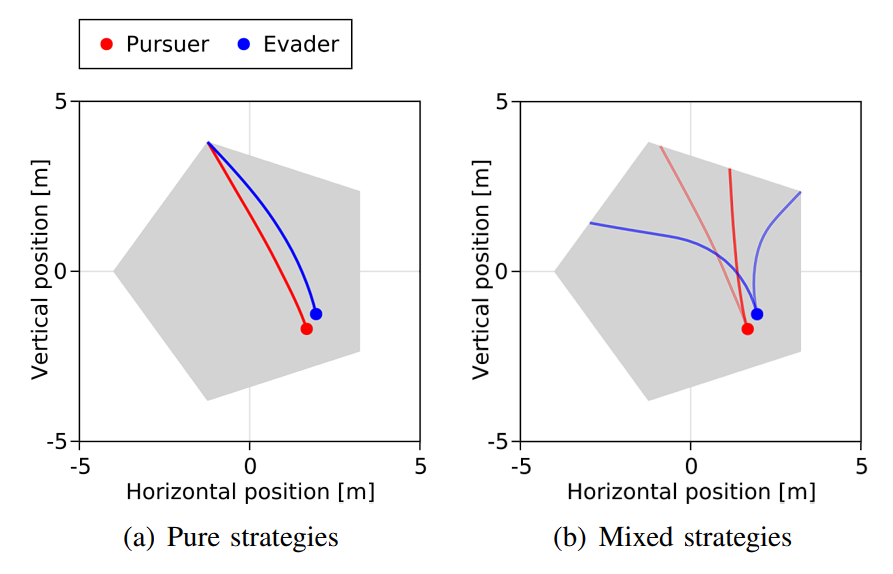
\includegraphics[width = 0.5\textwidth]{pres_images/pure_mixed_strats.png}
        \caption{Zero-sum game between 2 agents}
        \label{fig:zero_sum_pursuit_evasion}
    \end{figure}
    % 
    \footnotesize 
    [1] Peters, L., Fridovich-Keil, D., Ferranti, L., Stachniss, C., Alonso-Mora, J., \& Laine, F. (2022). Learning mixed strategies in trajectory games. arXiv preprint arXiv:2205.00291.
    
\end{frame} 

\begin{frame}{Overview}

    \begin{columns}
        \column{0.5\textwidth}
        Our goal is to extend the planar zero-sum pursuit-evasion game between two agents into a 3-dimensional game subject to orbital dynamics constraints.

        \column{0.5\textwidth}
        \begin{figure}
            \centering
            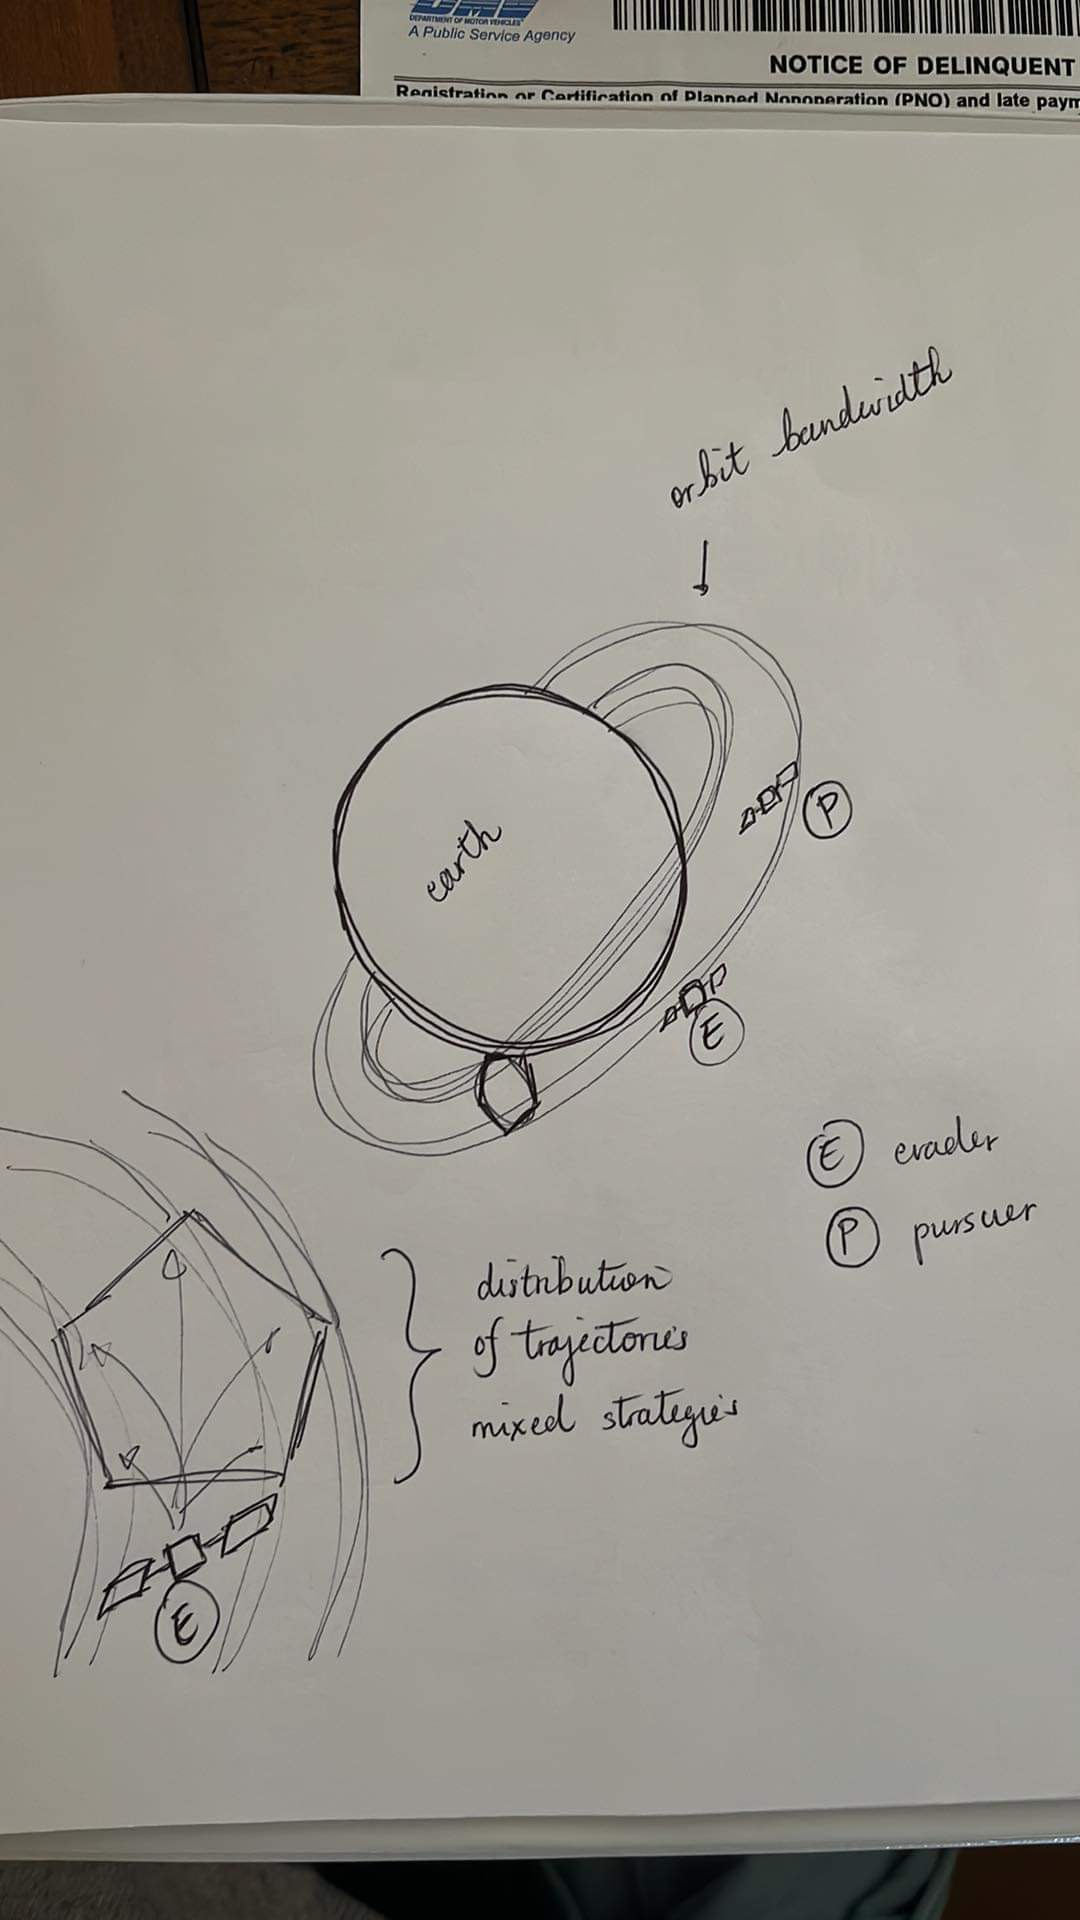
\includegraphics[height=0.7\textheight]{pres_images/polygon_tube.jpeg}
            \caption{Spacecraft Mixed Strategies}
            \label{fig:space_mixed}
        \end{figure}
    \end{columns}
    
\end{frame}



% \begin{frame}{Overview}
%         % \color{red}\rule{\linewidth}{4pt}
%     Our goal is to extend the planar zero-sum pursuit-evasion game between 2 agents into a 3-dimensional game subject to orbital dynamics constraints

% % \end{frame}

% % \begin{frame}{Overview}

%     \begin{figure}
%         \centering
%         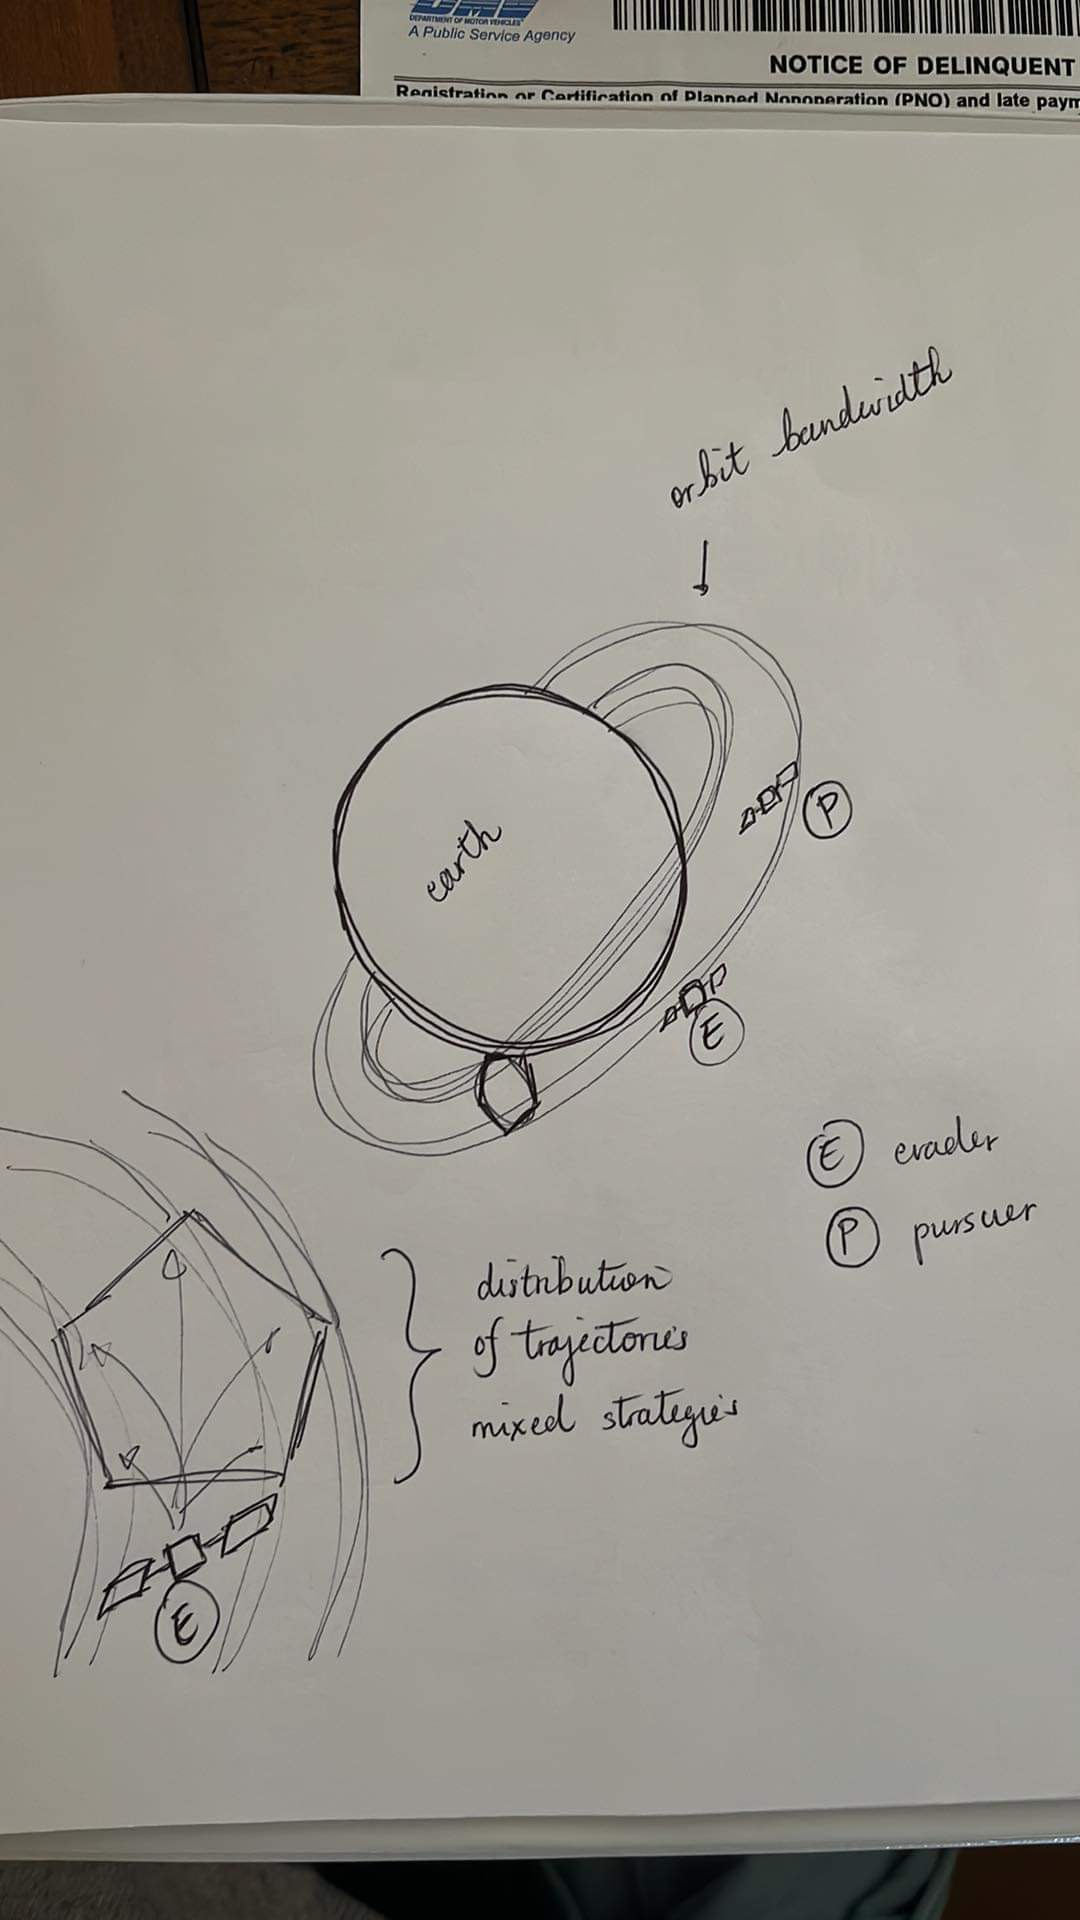
\includegraphics[height = 0.7\textheight]{pres_images/polygon_tube.jpeg}
%         \caption{Spacecraft Mixed Strategies}
%         \label{fig:space_mixed}
%     \end{figure}
    
% \end{frame}

